\documentclass[a4paper,11pt]{article}
\usepackage[margin=1in]{geometry}
\usepackage[czech]{babel}
\usepackage{amsmath}
\usepackage{csquotes}

% package na vklad obrázků
\usepackage{graphicx}
\usepackage{caption}
\usepackage{subcaption}
\usepackage{stfloats} % opravuje obrázky přes celou stránku
\graphicspath{ {./images/} } % definování složky s obrázky

% zvyšování hloubky obsahu
\setcounter{tocdepth}{4}
\setcounter{secnumdepth}{4}

% citace
\usepackage[
    citestyle=numeric,
    autocite=superscript,
    sorting=none
]{biblatex}
% \usepackage{biblatex}
\addbibresource{literature.bib}

\DeclareCiteCommand{\supercite}[\mkbibsuperscript]
{\iffieldundef{prenote}
{}
{\BibliographyWarning{Ignoring prenote argument}}%
\iffieldundef{postnote}
{}
{\BibliographyWarning{Ignoring postnote argument}}%
\bibopenbracket}%
{\usebibmacro{citeindex}%
\usebibmacro{cite}}
{\supercitedelim}
{\bibclosebracket}

\usepackage{listings}
\usepackage{xcolor}

\definecolor{backcolor}{rgb}{0.9, 0.9, 0.87}

\usepackage{siunitx}
\usepackage{color}

% abstrakt s větším písmem (https://tex.stackexchange.com/a/366170)
\makeatletter
\renewenvironment{abstract}{%
    \if@twocolumn
    \section*{\abstractname}%
    \else %% <- here I've removed \small
    \begin{center}%
    {\bfseries \Large\abstractname\vspace{\z@}}%  %% <- here I've added \Large
    \end{center}%
    \quotation
    \fi}
    {\if@twocolumn\else\endquotation\fi}
\makeatother

\selectlanguage{czech} % nastavení jazyka
\include{hyphenation} % upřesnění slabik v různých cizích slovech

\begin{document}

    %%% -------------------- Titulní strana --------------------
\begin{titlepage}
    \begin{center}
        \large \vspace*{\fill}
        \thispagestyle{empty}

        \LARGE

        { \huge \textbf{Gymnázium Arabská, Praha 6, Arabská 14}}

        {\LARGE Obor programování }

        \vfill
        
\includegraphics{logogyarab.png}
        \vspace{15pt}

        \vfill

        {\huge \textbf{Neuronová síť: Digitor}}

        \vfill

        Ondřej Salát

        \vfill

        {\large Duben, 2024}

        \vspace*{\fill}
    \end{center}
\end{titlepage}

%%% -------------------- Prohlášení --------------------
\thispagestyle{empty}
\addtocounter{page}{-1}
\vspace*{\fill}
Prohlašuji, že jsem jediným autorem tohoto projektu, všechny citace jsou řádně označené a všechna
použitá literatura a další zdroje jsou v práci uvedené.
Tímto dle zákona 121/2000 Sb. (tzv.\ Autorský zákon)
ve znění pozdějších předpisů uděluji bezúplatně škole Gymnázium, Praha 6, Arabská 14 oprávnění k výkonu
práva na rozmnožování díla (§ 13) a práva na sdělování díla veřejnosti (§ 18) na dobu časově neomezenou a
bez omezení územního rozsahu.

\vspace{2cm}
V .......... dne ............... \hspace{4cm} Ondřej Salát .................

\vspace{2cm}

%%% -------------------- Anotace --------------------
\newpage
\begin{abstract}
    Práce se zabývá procesem tvorby programu na vytváření a trénování neuronových sítí.
    Popisuje princip strojového učení za použití algoritmu backpropagation.
    Dále se práce věnuje pokusu o hlubší pochopení neuronových sítí.
    Konkrétně se věnuje různým architekturám neuronové sítě pro rozpoznávání rukou napsaných cifer.
\end{abstract}

%%% -------------------- Obsah --------------------
\tableofcontents  % povinné strany

    \section{Úvod}
Cílem maturitní práce je vytvořit neuronovou síť a naprogramovat k ní základní učící algoritmus bez použití knihoven pro strojové učení (jako TensorFlow, nebo PyTorch).
Záměrem je hlubší pochopení a prozkoumání různých implementací neuronových sítí.
Neuronová síť Digitor bude natrénována pro rozpoznávání rukou napsaných číslic [0-9].
Síť dostane na vstup čtvercový obrázek a výstupem bude číslice obsažena v obrázku.

\subsection{Výběr tématu}
Toto téma jsem si vybral z důvodu, že si myslím, že neuronové sítě jsou velice zajímavé a dosud ne úplně prozkoumané téma.
Věřil jsem, že tvorbou tohoto projektu se naučím jak neuronové sítě fungují.
Zárověn bych na toto téma rád navázal při studiu na vyskoké škole.
    \section{Neuronová síť}
Neuronová síť je výpočetní model, který je inspirován fungováním lidského mozku.
Neuronová sít se skláda z tzv. umělých neuronů a váh.
Neurony jsou propojeny váhami mezi vrstvami.

Struktura neuronové sítě:
\begin{itemize}
    \item vstupní vrstva - zde se zadají vstupní data
    \item skryté vrstvy - tyto vrstvy transofrmují data a napomáhají řešit komplexní úlohy
    \item výstupní vrstva - vrací výsledky zpracování dat
\end{itemize}

Počty neuronů v každé vrstvě závisí na konkrétním využití a na problému, který má neuronová síť řešit.

Každý neuron představuje jednoduchý výpočetní prvek, který zpravová vstupy a generuje výstup.
Vstupy a výstupy jsou spojeny váhami, které ovlivňují hodnoty neuronů, ze kterých váha vede.
Dále má každý neuron svůj bias, který ovlivňuje jeho hodnotu.

\begin{figure}[h]
    \centering
    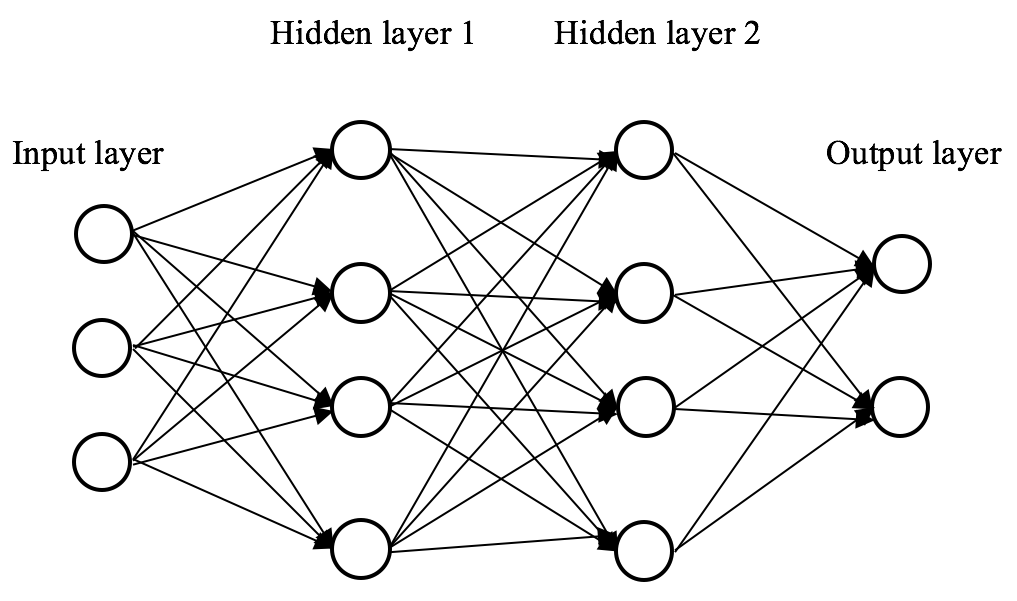
\includegraphics[width=0.75\textwidth]{images/network.png}
    \caption{Neuronová síť}\cite{sit}
\end{figure}

Existují různé typy neuronových sítí, které se liší tím, jak jsou neurony mezi vrstvami propojeny.
Různé typy propojení jsou vhodné pro různé typy úloh.
Mezi nejběžnější typy patří neuronové sítě typu perceptrony, vícevrstvé perceptory, konvulační neuronové sítě a rekurentní neuronové sítě.

Mezi hlavní výhody neuronových sítí patří schopnost učit se z dat a adaptovat se novým informacím.
Neuronové sítě dokáží řešit komplexní úlohy, které jsou extrémně náročné pro běžné algoritmy.
Tyto sítě jsou také vhodné pro práci s velými objemi dat.

\subsection{Fungování neuronových sítí}
Neuronová síť načte vstup a postupně se počítají hodnoty neuronů po vrstvách.
Až hodnoty projdou celou sítí nakonec, ve výstupní vrstvě je výsledek.

Hodnota konkrétního neuronu se spočítá z jeho vstupů. Každý neuron, až na vstupní vrstvu, má vstupní neurony.
Jeho hodnota se vypočíta ta, že se sečte hodnota všech jeho vstupních neuronů vynásobena spojujícími vahami každého neuronu.
Dále se přičte bias daného neuronu, který slouží jako práh aktivace. Nakonec se použije aktivační funkce.
Aktivačních funkcí je řada. Mezi nejběžnější patří například sigmoid nebo ReLU. Výběr ideální aktivační funkce opět zavisí na problému, který má síť řešit.
Tyto funkce v jednoduchosti transformují vstupy neuronu na jeho výstupy.
Aktivační funkce dodávají sítím jistou nelinearitu, která umožňuje sítím řešit i problémy, které nejsou linearní.

\begin{figure}[h]
    \centering
    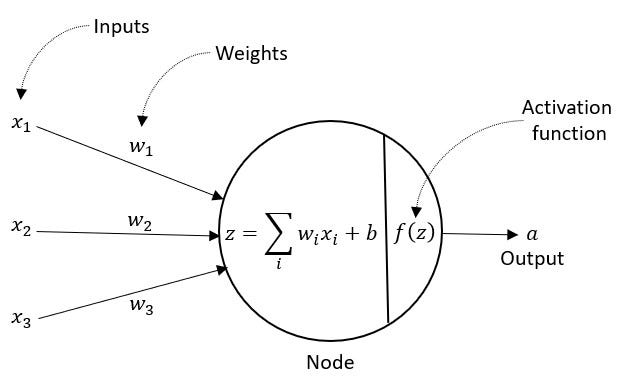
\includegraphics[width=0.75\textwidth]{images/neuron.jpg}
    \caption{Umělý neuron}\cite{umely_neuron}
\end{figure}

\subsection{Implementace v programu}



    \section{Strojové učení}
Strojové učení je nedílnou součástí celé kapitoly neuronových sítí. Strojové učení se umožňuje sítím se učit ze známých dat.
Díky strojovému učení je možné řešit problémy, které byly do objevení těchto učících technik neřešitelné.
Existuje několik způsobů učení, ale v této práci bylo použito takzvané učení s učitelem.
To znamená, že všechny data, ze kterých se síť učí jsou předkládána síti se správným výsledkem.
Existují však metody bez učitele, které se dokáží učit i z nepopsaných dat.

Princip storjového učení je,že síť dostane data se správnými výsledky a síť si na základě těchto dat poupraví svoje hodnoty vah a biasů tak,
aby při načtení těchto dat odpověděla příště správně.

\subsection{Zpětné počítání chyby}
Zpětné počítání chyby\cite{backpropagation}, neboli backpropagation, je algoritmus pro hluboké učení neuronových sítí.
Tento algoritmus funguje tak, že se šíří chyba výstupu zpátky do neuronové sítě a podle chyby upravuje postupně váhy a biasy.

Tento algoritmus se skládá ze 4 kroků. Nejprve se musí vyhodnotit chyba. To znamená, že se konkrétní dat nechají vyhodnotit sítí a spočítá se chyba.
Chyba je v tomto případě rozdíl od očekávaného výsledku. Dále se chyba šíří zpět do sítě a počítá se derivace chyby vzhledem ke konkrétním vahám a biasům.
Na základě této derivace se váhy a biasy aktualizují. Tato aktualizace pomáhá zmírňovat celkovou chybu výsledku. Nakonec se tento proces pro všechny trénovací data opakuje.

\subsection{Počítání chyby a aktualizace vah a biasů}
Celková chyba sítě se označuje velkým písmenem \(C\). Při zpětné úpravě vah a biasů nás zajímá jaká je derivace chyby vůči každé váze \(\frac{\delta C}{\delta w}\) a biasu \(\frac{\delta C}{\delta b}\).
V moment, kdy budeme znát tento vztah, tak víme jakým směrem upravit váhu nebo bias, abychom snížili celkovou chybu sítě.

Důležitá část pro pochopení vzorce algoritmu zpětné počítání chyby je notace zápisu neuronové sítě.
Proto je potřeba nejprve definovat zápis a až dále se budu věnovat samotným vzorcům a vztahům při počítání zpětné počítání chyby.
Pro po popsání váhy budem zapisovat jako \(w_{jk}^l\), kde \(l\) je číslo vrstvy, \(j\) je označení,
do kterého neuronu v \(l\)-té vrstvě váha směřuje a číslo \(k\) označuje z kolikátého neuronu z vrstvy \((l-1)\) váha vychází.

\begin{figure}[h]
    \centering
    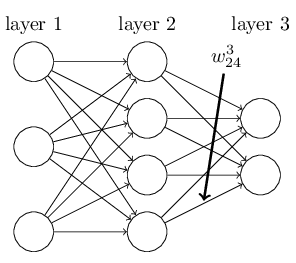
\includegraphics[width=0.4\textwidth]{images/vaha_v_siti.png}
    \caption{Příklad zápisu váhy}\cite{vaha_v_siti}
\end{figure}

Podobná notace se použije také při popisu biasu, neaktivované a neaktivované hodnoty neuronu.
Bias neuronu se zapíše jako \(b_{j}^l\), kde \(l\) je vrstva neuronu a \(j\) je \(j\)-tý neuron v \(l\)-té vrstvě.
Hodnota neuronu před aktivací je označí písmenem \(z_{j}^{l} = \left( \sum (w^{l}_{jk} a^{l-1}_k) + b^l_j \right)\).
Hodnota aktivovaného neuronu ze zapíše jako \(a_j^l = \sigma(z_j^l)\).

\begin{figure}[h]
    \centering
    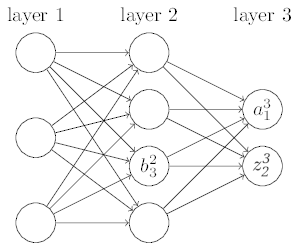
\includegraphics[width=0.4\textwidth]{images/bias_a_neuron.png}
    \caption{Příklad zápisu biasu, aktivace a neaktivace neuronu} \cite{bias_a_neuron}
\end{figure}


    \section{Implementace v programu}
Program slouží k vytváření a trénování neuronových sítí podle vstupních parametrů.
Samotný program se dá spustit s přepínači, které určují chování programu.
Program je schopen na požadavek buď vytvořit novou síť podle vstupních parametrů, nebo načíst existující síť ze souboru JSON.
S takto vytvořenou neuronovou sítí je program dále schopen pracovat dvěma způsoby.
Neuronovou síť může trénovat nebo jí jen načte a čeká na vstupní data, která neuronová síť zpracuje a vrátí výsledek.

\subsection{Vytváření a načítání neuronové sítě}
Neuronová síť je v programu reprezentována vícerozměrnými poli. První dvojrozměrné pole reprezentuje neurony.

Pole \(neuron\) má dva rozměry tzn. pole v poli.
První (nulté) pole v \(neuron\) reprezentuje první vrstvu neuronů (vstupní) vrstvu.
Naopak poslední prvek pole \(neuron\) reprezentuje poslední (výstupní) vrstvu.
Počet skrytých vrstev v neuronové síti se tedy rovná \(neuron.size() - 2\).
Každé toto pole uložené v \(neuron\) obsahuje \(n\) hodnot, které reprezentují hodnoty konkrétních neuronů. Hodnoty jsou typu long double.

Dále je potřeba pole \(rawNeuron\), které je úplně stejné jako pole \(neuron\), ale jsou do něj ukládány neaktivované hodnoty neuronů.

Další pole \(bias\) má také dva rozměry a jeho velikost je identická jako velikost pole \(neuron\).
Hodnoty v jednotlivých polích reprezentují hodnotu biasu konkrétního neuronu. Hodnoty jsou také typu long double.

Poslední pole reprezentující samotnou neuronovou síť je trojrozměrné pole \(weight\). Velikost pole je rovno počtu vrstev mínus jedna.
První (nultý) prvek tj. \(weight[0]\) reprezentuje dvojrozměrné pole, které reprezentuje váhy spojující vstupní neurony s neurony druhé vrstvy.
Pole \(weight[0][0]\) je pole hodnot jednotlivých vah, které míří do prvních (nultého) neuronu druhé vrstvy. Váhy jsou také typu long double.

Při vytváření nové neuronové sítě se v konstruktoru vytvoří zmiňovaná pole o velikostech, které odpovídají zadaným parametrům.
Hodnoty vah a biasů se incializují s náhodnou hodnotou. Dále se celá neuronová síť serializuje do souboru JSON, který se následně uloží.
V názvu souboru je obsažen počet vrstev sítě navíc s náhodným číslem, které se pokusí zabránit kolizi na disku.
Soubor obsahuje všechna potřebná data pro pozdější načtení neuronové sítě.
To znamená velikost, aktivační funkce neuronů, hodnoty vah a hodnoty biasů.

Pokud program pouze načítá neuronovou síť z již existujícího souboru, konstruktor pouze očekává název souboru.
Dále konstruktor deserializuje data ze souboru a uloží si je do proměnných.

\subsection{Trénování neuronové sítě}
Jak už bylo zmíněno v kapitole o strojovém učení, proces učení neuronové sítě se skládá ze čtyř částí. Tedy průchod dat sítí a vyhodnocení chyby,
zpětné počítání chyby, aktualizace vah a biasů a nakonec se vše zopakuje. Průchod dat sítí neboli přímý průchod je vyřešen jako tři vnořené \(for\) cykly.
Hodnota každého neuronu se vypočítá podle vzorce na výpočet hodnoty neuronu, a tudíž \(z_{j}^{l} = \left( \sum (w^{l}_{jk} \cdot a^{l-1}_k) + b^l_j \right)\).
Z důvodu, že při zpětném počítání chyb je potřeba aktivovaný i neaktivovaný neuron, tak se do paměti uloží obě hodnoty (do pole \(neuron\) a \(rawNeuron\)).
Pro samotné učení je v programu metoda \(train\), která všechny tyto kroky provede.

Při volání metody \(train\), funkce očekává dvojrozměrné pole typy \(TrainData\), které obsahuje vstupní hodnoty a správný výsledek průchodu,
počet trénovacích cyklů (iterací) a jako poslední parametru očekává tzv. rychlost učení (learning rate).
Learning rate určuje míru změny při aktualizaci vah a biasů. Hodnota rychlosti učení se běžně pohubuje v rozmezí od 0.1 do 0.0001.
Pole \(TrainData\) je dvojrozměrné z důvodu, že data jsou rozdělena do tzv. seté, které zajišťují rychlejší a univerzálnější učení.
Tím pádem metoda \(train\) funguje tak, že zavolá metodu \(backpropagate\) na všechny členy setu.
Aktualizované hodnoty vah a bíasů se ukládají do externího pole a skutečné váhy a biasy neuronové sítě se aktualizují až po dokončení.
Takto se postupně trénuje síť pomocí všech setů dat. Následně se celý tento proces opakuje podle počtu iterací.
Metoda v průběhu počítá průměrnou chybu pro vstupní data, kterou vypisuje na standardní výstup společně s progresem trénování (procento vykonaných iterací).

Metoda \(backpropagate\) funguje na principu popsaném v kapitole \ref{strojove_uceni} Strojové učení. Funkce je rozdělena do dvou částí.
První část spočíta chybu pro poslední vrstvu, která se počítá jednodušeji, protože neurony ovlivňují chybu pouze jednou cestou.
Druhá část naváže na první a počítá zpětně chybu pro zbytek vrstev. Pro výpočty jsou použity vzorce z kapitoly \ref{strojove_uceni} o strojovém učení.

\subsection{Spouštění programu}
Při spouštění si pomocí přepínačů lze nastavit, zda chceme například vytvářet úplně novou neuronovou síť, nebo chceme načíst již exístující síť. Dále je možné specifikovat jestli chceme síť trénovat nebo ji chceme použít k zpracování dat.

Možné použití jsou:
\begin{itemize}
    \item Načte neuronovou síť ze souboru a čeká na standartním vstupu data na zpracování.
    \begin{lstlisting}[language=bash, backgroundcolor=\color{backcolor}]
 $ ./digitor <jmeno_souboru>
    \end{lstlisting}

    \item Vytvoří neuronovou síť podle zadaných parametrů.
    Formát pro zadání neuronů je vždy počet neuronů pro každou vrstvu, který je oddělen čárkou.
    Př. "10,2,2,10", tato síť by měla čtyři vrstvy, z čehož vstupní i výstupní by měla 10 neuronů a obě skryté by měly 2 neurony.
    \begin{lstlisting}[language=bash, backgroundcolor=\color{backcolor}]
 $ ./digitor -n <neurony> <aktivace>
    \end{lstlisting}

    \item Trénování exitující sítě. Program dostane informace o počtu učících dat, počtu iterací a míře učení.
    Dále program čeká na standartní vstup zmiňované učící data a následovně síť trénuje.
    \begin{lstlisting}[language=bash, backgroundcolor=\color{backcolor}]
 $ ./digitor -t <jmeno_soubor> <pocet_iteraci> <rychlost_uceni>
    <pocet_davek> <pocet_dat>
    \end{lstlisting}

    \item Vytvoří novou neuronovou síť podle požadavků a síť natrénuje stejným způsobem jako v předešlém bodě.
    \begin{lstlisting}[language=bash, backgroundcolor=\color{backcolor}]
 $ ./digitor -t -n <neurony> <iterace> <rychlost_uceni>
    <aktivace> <pocet_davek> <pocet_dat>
    \end{lstlisting}
\end{itemize}
\newpage
    \section{Zkoumání architektur}
Při vytváření sítě na rozpoznávání rukou napsaných číslic jsem narazil na problém, že nevím, jak velkou sít mám použít.
Při hledání na internetu jsem zjistil, že vlastě neexistuje žádná perfektní síť, a že ideální velikost sítě vždy závisí na problému, který má řešit.
Z toho důvodu jsem se rozhodl, že vytvořím malý výzkum na to, které síť má nejlepší výsledky.
Vytvořil jsem proto osm různých neuronových sítí, kterým jsem dal úplně stejný učící set a stejný počet iterací na natrénování.
Sítě měly vždy stejný počet vstupních a výstupních neuronů pouze se lišily v počtu skrytých vrstev a v počtu neuronů v těchto vrstvách.
Použité architektury byly následovné:
\begin{itemize}
    \item 2 vrstvy po 64 neuronech
    \item 3 vrstvy po 16 neuronech
    \item 3 vrstvy po 24 neuronech
    \item 3 vrstvy po 32 neuronech
    \item 3 vrstvy po 40 neuronech
    \item 3 vrstvy po 48 neuronech
    \item 3 vrstvy po 56 neuronech
    \item 3 vrstvy po 64 neuronech
\end{itemize}
Tyto konkrétní architektury jsem zvolil z důvodu, že se mi ještě před uskutečněním tohoto zkoumání podařilo vytvořit model,
který měl 3 skryté vrstvy po 64 neuronech, a který dokázal rozpoznat obrázky s vysokou přesnotsí.
Proto mě napadlo zkusit, kolik neuronů je potřeba, aby neuronová síť měla uspokujivé výsledky.
Zvolil jsme tedy neuronové sítě, které mají postupně nižsí počet neuronů a zkoumal jsem, jaký to má vliv na výsledky.

Vytvořil jsem tedy 8 těchto sítí a spustil jsme trénování. Všechný sítě dostaly identická data a identický počet iterací.
Zárověň jsem měřil čas, za jak dlouho se síť s těmito parametry natrénuje. Sítě byly tedy na trénovány pomocí 10000 obrázků (1000 z od každé číslice).
Po ukončení trénování jsem sítě otestoval pomocí 27730 vyčleněných obrázků z databáze mnist, které sítě nikdy neviděly.

\begin{center}
    \begin{tabular}{||c c c||}
        \hline
        Architektura        & Čas učení   & Přesnost \\ [0.5ex]
        \hline\hline
        2 vrstvy 64 neuronů & 20h 5m 31s  & 53.0\%   \\
        \hline
        3 vrstvy 16 neuronů & 5h 46m 27s  & 24.7\%   \\
        \hline
        3 vrstvy 24 neuronů & 8h 30m 19s  & 34.6\%   \\
        \hline
        3 vrstvy 32 neuronů & 10h 42m 14s & 54.5\%   \\
        \hline
        3 vrstvy 40 neuronů & 13h 49m 14s & 50.9\%   \\
        \hline
        3 vrstvy 48 neuronů & 16h 48m 6s  & 57.9\%   \\
        \hline
        3 vrstvy 56 neuronů & 19h 54m 12s & 55.2\%   \\
        \hline
        3 vrstvy 64 neuronů & 23h 25m 54s & 58.4\%   \\
        \hline
    \end{tabular}
\end{center}

Z výsledků je zřejmé, že sítě s vyšším počtem neuronů mají v tomto případě lepší výsledky, ale trénování takových sítí trvá déle.
V tomto připadě jsem došel k závěru, že rozdíl mezi trénováním menších a větších sítí není tak markantní,
a tudíž se v tomto konkrétním připadě vyplatí použít sítě s většim počtem vrstev a neuronů.
Největší síť se dokázala vytrénovat v pozdějším trénování vytrénovat natolik, že dokázala poznat více než 98\% obrázků, které nikdy neviděla.
    \section{Závěr}
Při vytváření tohoto projektu jsem se ponořil do problematiky neuronových sítí a zjistil jsem na jakém principu funguje strojové učení pomocí zpětného počítaní chyby.
Tento projekt mi pomohl vytvořit si představu jak neuronové sítě fungují a k čemu vůbec mohou sloužit.

\subsection{Prostor pro zlepšení}
V budoucnu bych chtěl v programu implementovat parelelní výpočet pomocí CUDA. Díky tomu by se mohlo trénování sítí řádově urychlit.
Dále bych chtěl v budoucnu přidat možnost pro vytváření jiných typů neuronových sítí než jen plně propojených.

    \newpage
    \printbibliography
    \listoffigures

\end{document}